\chapter{Architecture}

\section{Présentation de l'architecture du projet}
\subsection{Diagramme de flux des données}

\begin{figure}[H]
  \centering
    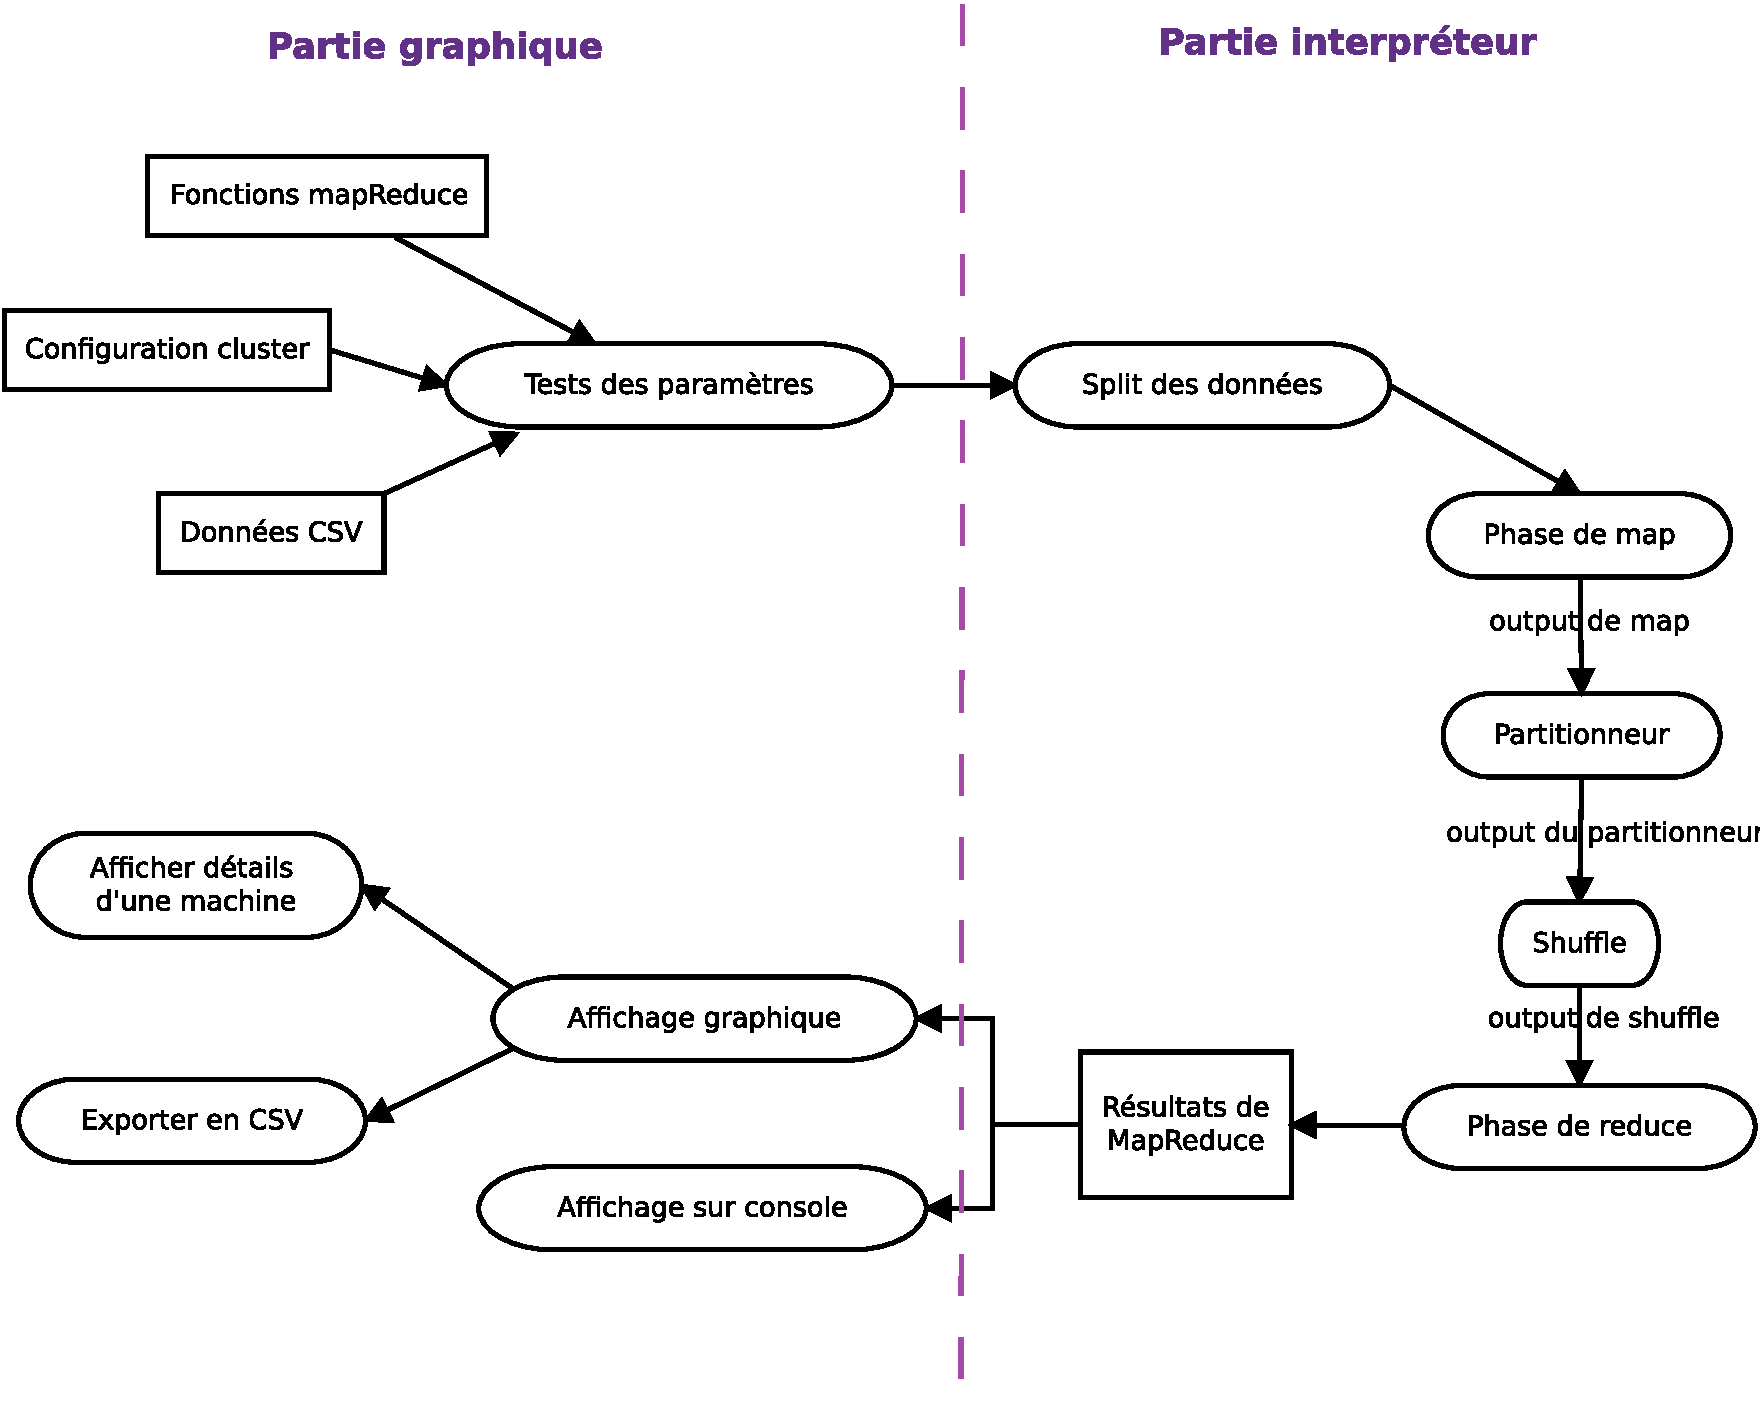
\includegraphics[width=1\textwidth]{diagram/dfd.pdf}
        \caption{Diagramme de flux des données}
        \label{fig:dfd}
\end{figure}
\newpage
Ce diagramme de flux (Figure: \ref{fig:dfd}) des données résume le passage des données en entrée dans une {\it boite noire} pour ensuite récupérer le résultat final en sortie. Lorsque l'application est lancée, les données sont traitées dans la partie graphique (zone de gauche) puis sont envoyées à la partie interpréteur (zone de droite).

\subsection{Architecture client-lourd | 2-tiers}
Notre projet consiste en un site web qui ne possède pas de base de données. Le serveur ne sert qu'a accéder à son URL\footnote{Uniform Resource Locator} c'est-à-dire qu'il n'est utilisé que pour héberger le contenu du site. Le traitement dans sa totalité se fait du coté du navigateur directement et aucune donnée n'est envoyée/conservée ou reçue d'un serveur.
Ce type d'application correspond donc à l'architecture {\bf Client-lourd}.

D'autre part, on remarque que ce projet peut être divisé en deux parties indépendantes, l'une qui va traiter l'exécution de {\it MapReduce}, et l'autre qui s'occupe du coté visuel/graphique. On parle ici d'une séparation entre le {\it traitement} et {\it l'affichage graphique}.

Nous avons donc eu l'idée de suivre l'architecture {\bf 2-couches} pour représenter cette séparation.

Ainsi, notre projet présente une architecture {\bf client-lourd | 2-tiers} combinées pour améliorer l'organisation du travail. Chaque couche est constituée de plusieurs composants comme précisé dans la figure \ref{fig:clientlourd}. Nous détaillerons dans le prochain chapitre les différents composants.

 \begin{figure}[H]
  \centering
    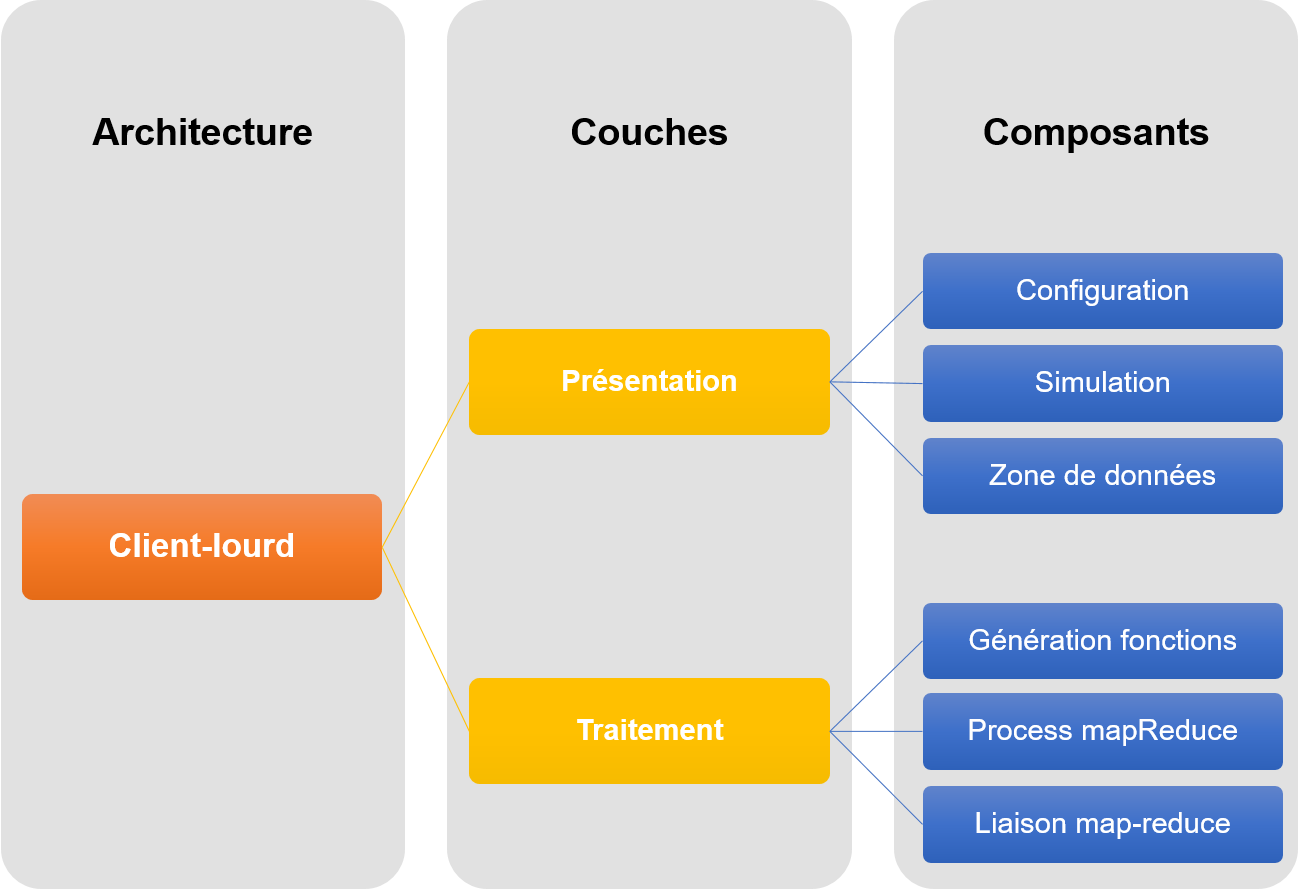
\includegraphics[width=0.81\textwidth]{images/clientlourd.png}
        \caption{Architecture client lourd | 2-tiers}
        \label{fig:clientlourd}
\end{figure}
\newpage
\subsection{Diagrammes de séquence} 

Le diagramme de séquence (Figure \ref{fig:seq}) montre les étapes de déroulement du programme. L'utilisateur interagit avec l'interface graphique. Les entrées qu'il fournit sont transmises à l'interpréteur qui lui effectue le traitement nécessaire et renvoie un résultat de la simulation. Sur la simulation obtenue, l'utilisateur peut voir la section de données prise en charge par la machine qu'il consulte. La partie d'exportation des données en code Java est un besoin optionnel que nous n'avons pas réussi à implémenter.

 \begin{figure}[H]
  \centering
    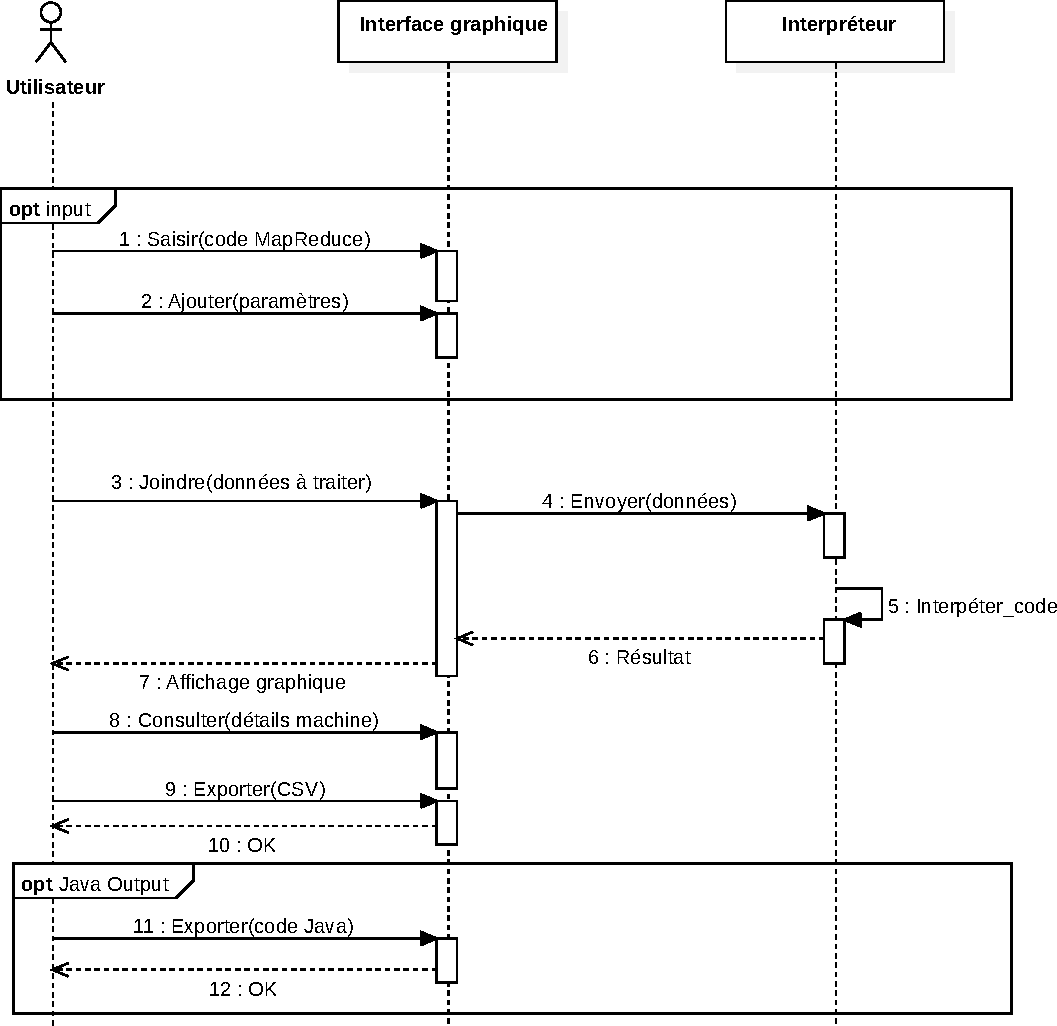
\includegraphics[width=1\textwidth]{diagram/SequenceDiagram.pdf}
        \caption{Diagramme de séquence}
        \label{fig:seq}
\end{figure}
